\documentclass{article}
\usepackage[T2A]{fontenc}
\usepackage[utf8]{inputenc}
\usepackage[english, russian]{babel}
\usepackage[left=3.5cm,right=3.5cm]{geometry}
\usepackage[center]{caption}
\usepackage{graphicx}
\usepackage{subfig}
\usepackage{float}
\usepackage{indentfirst}
\usepackage{amsmath}
\usepackage{amssymb}
\usepackage{hyperref}
\usepackage{fontawesome}
\usepackage{array}
\usepackage{bm}

\hypersetup{
    colorlinks=true,
    linkcolor=black,
    urlcolor=black,
}
\urlstyle{same}

\makeatletter
\renewcommand{\@biblabel}[1]{#1.}
\makeatother
\newcommand{\bibref}[3]{#2\hyperlink{#1}{\color{blue}#3}}
\newcolumntype{M}[1]{>{\centering\arraybackslash}m{#1}}
\renewcommand{\baselinestretch}{1.2}

\newcommand{\R}{\mathbb{R}}
\newcommand{\norm}[1]{\left\lVert#1\right\rVert}

\begin{document}

\begin{center}
    \textbf{{\huge Случайные признаки в машинном обучении}} \href{https://github.com/isadrtdinov/random-features}{\Large \faGithub} \\
    \vspace{10pt}
    {\Large И.Р. Садртдинов, Е.М. Шабалин}
\end{center}{}

\vspace{1cm}

Многих алгоритмы машинного обучения так или иначе используют случайность. Это может быть, например, бутстрэп в случайных лесах или случайная инициализация весов нейросетей. В этой работе мы разберем подход, основанный на использовании рандомизированных признаков. Конечно, случайности сложно соперничать с общепризнанными гигантами среди моделей вроде градиентного бустинга или многослойных нейросетей, но оказывается, что применение рандомизированного подхода может привести к улучшению качества моделей. 

\section{Random Fourier Features (RFF)}

Использование ядрового перехода позволяет использовать нелинейные преобразования признаков, что приводит к снижению смещения моделей. Однако, введение ядер заметно усложняет вычислительную сложность обучения и применения алгоритмов. Здесь на помощь приходит теорема Бохнера, и некоторые ядра (инвариатные относительно сдвига, shift-invariant kernels) удается представить через преобразование Фурье по определенному вероятностному распределению (будем считать, что $x, y \in \R^d$). 

$$
K(x, y) = K(x - y) = \int_{\R^d} e^{i w^T (x - y)} p(w) dw = \int_{\R^d} \cos \left(w^T (x - y) \right) p(w) dw
$$

\noindent
Этот интеграл можно оценить методом Монте-Карло. Если преобразовать косинус разности, можно перейти к скалярному произведению объектов в некотором другом пространстве.

$$
K(x - y) = \mathbb{E}_{w \sim p} \Big[\cos \left(w^T (x - y) \right)\Big] \approx \sum_{i=1}^D \cos \left(w^T_i (x - y) \right) = 
$$

$$
= \sum_{i=1}^D \cos \left(w_i^T x\right) \cos \left(w_i^T y\right) + \sin \left(w_i^T x\right) \sin \left(w_i^T y\right)
$$

\noindent
Новые признаковые описания выглядят так (тут вводится нормализация с помощью 
деления на $\sqrt{D}$).

$$
\widetilde{x} = \frac{1}{\sqrt{D}} \Big[\cos \left(w_1^T x\right), \dots, \cos \left(w_D^T x\right), \sin \left(w_1^T x\right), \dots, \sin \left(w_D^T x\right) \Big]
$$

\noindent
Получаем аппроксимацию ядра:

$$
K(x - y) \approx \langle \widetilde{x}, \widetilde{y} \rangle
$$

Однако на практике лучший результат показывают признаки, сконструированные немного по-другому. Поскольку $\sin \alpha = \cos \left(\alpha - \frac{\pi}{2}\right)$, то синусы можно аппроксимировать, добавив в косинусы внутренние сдвиги $b_i$, распределенные равномерно на $[-\pi, \pi]$:

$$
\overline{x} = \sqrt{\frac{2}{D}} \Big[\cos \left(w_1^T x + b_1\right), \dots, \cos \left(w_D^T x + b_D \right)\Big]
$$

\noindent
В дальнейшем число случайных признаков будем обозначать за $D$. В итоге преобразование в новое признаковое пространство выглядит так:

$$
\widetilde{x} = \cos \left(Wx + b\right)
$$

$$
W \in \R^{D \times d}, W_i \sim p \quad\quad\quad b \in \R^D, b_i \sim U[-\pi, \pi]
$$

\subsection{Алгоритм}

В статье \bibref{kernels}{}{Ali Rahimi, Benjamin Recht} приводятся распределения для трех ядер.

\begin{table}[H]
\centering
    
\begin{tabular}{M{2cm}|M{3cm}M{3cm}}
    Ядро & $K(\Delta)$ & $p(w)$ \\
    \hline
    Гаусс & $e^{-\frac{{\norm{\Delta}^2_2}}{2}}$ & $(2\pi)^{-\frac{d}{2}}e^{-\frac{{\norm{w}^2_2}}{2}}$ \\
    Лаплас & $e^{-{\norm{\Delta}_1}}$ & $\prod_i \frac{1}{\pi \left(1 + w_i^2\right)}$ \\
    Коши & $\prod_i \frac{2}{1 + \Delta_i^2}$ & $2^{-d} e^{-{\norm{w}_1}}$
\end{tabular}

\label{tab:my_label}
\end{table}

В первую очередь необходимо оценить дисперсию для этих распределений. Обозначим за $\mathbb{X}$ распределение объектов выборки. Обозначим за $s$ среднюю норму разности между объектами выборки, оценим ее по некоторой подвыборке обучающей выборки. Параметр масштаба для всех распределений примем одинаковым и равным $\sigma = \frac{1}{s}$.

$$
s = \mathbb{E}_{x, y \sim \mathbb{X}} \Big[\norm{x - y}_2\Big] \approx \frac{1}{L^2} \sum_{i, j = 1}^L \norm{x_i - x_j}_2
$$

Затем сэмплируем случайную матрицу $W \in \R^{D \times d}$ и вектор сдвигов $b \in \R^D$. Каждый элемент матрицы можно просемплировать из соответствующего одномерного распределения (мы рассматриваем покомпонентно независимые многомерные распределения). Далее генерируем новые признаки $\widetilde{x} = \cos (Wx + b)$ и обучаем на них логистическую регрессию.

\subsection{Ортогональные признаки (ORF)}

Хорошо известно, что многие алгоритмы машинного обучения работают лучше, если признаки объектов нескоррелированы. Для случайных признаков можно добиться похожего эффекта. Разберем подробно этот подход на примере ядра Гаусса, описанный в статье \bibref{orf}{}{Felix Xinnan Yu et al}.

Пусть элементы матрицы $G \in \R^{d \times d}$ распределены по стандартному нормальному закону, $G_{ij} \sim \mathcal{N}(0, 1)$. Обычный метод случайных признаков Фурье использует матрицу $W = \sigma G$. Попробуем использовать случайную ортогональную матрицу $Q$, распределенную равномерно на множестве ортогональных матриц ($Q \sim U(O(d))$). Как известно, столбцы матрицы $Q$ образуют ортонормированный базис. Теперь можно было бы использовать матрицу $W = \sigma Q$, но такие признаки не будут аппроксимировать ядро Гаусса.

Дело в том, что нормы строк матрицы $G$ имеют хи-распределение:

$$
\norm{G_i}_2 = \sqrt{\sum_{j=1}^d G_{ij}^2} \sim \chi(d)
$$

\noindent
В то же время, нормы строк матрицы $Q$ равны $1$. Однако, можно уравнять распределения норм строк, если домножить матрицу $Q$ слева на диагональную матрицу $S$, распределенную по $\chi(d)$:

$$
S_{ij} = \begin{cases}
    s_i \sim \chi(d), & i = j \\
    0, & i \ne j
\end{cases}
$$

\noindent
Ортогональные признаки Фурье считаются по формуле $\widetilde{x} = \cos (Wx + b) = \cos (\sigma S Q + b)$.

Осталось выяснить, как генерировать случайную ортогональную матрицу $Q$. Утверждается, что можно взять случайную нормальную матрицу $G$, применить к ней QR-разложение, и получившаяся матрица $Q$ будет распределена равномерно на множестве ортогональных матриц.

Стоит отметить, что на практике $D \le d$ признаков недостаточно для получения хорошего качества, однако процедуру, описанную выше, можно повторить несколько раз, пока не будет получено желаемое число признаков. 


\subsection{Регуляризация}

Также мы вывели эмпирическую закономерность, которую можно использовать для регуляризации модели. Ранее мы вводили масштабирующий коэффициент как $\sigma = \frac{1}{s}$. Можно фиксировать некоторый параметр $\lambda$ и ввести параметр масштаба как $\sigma = \frac{\lambda}{s}$. С уменьшением разброса случайных признаков модели становится сложнее подгоняться под обучающую выборку. Этот эффект подтверждается экспериментами.

\section{Данные}

За основу мы взяли данные о классификации картин импрессионистов с \bibref{kaggle}{}{kaggle.com}. Данные содержат картины десяти художников, заранее разделенные на обучающую и валидационную выборку. При работе это разделение было сохранено. Для оценки качества мы использовали метрики accuracy и top-3 accuracy. Примеры картин из обучающей выборки представлены на рис. 1.

\begin{figure}[H]
    \centering
    \subfloat{{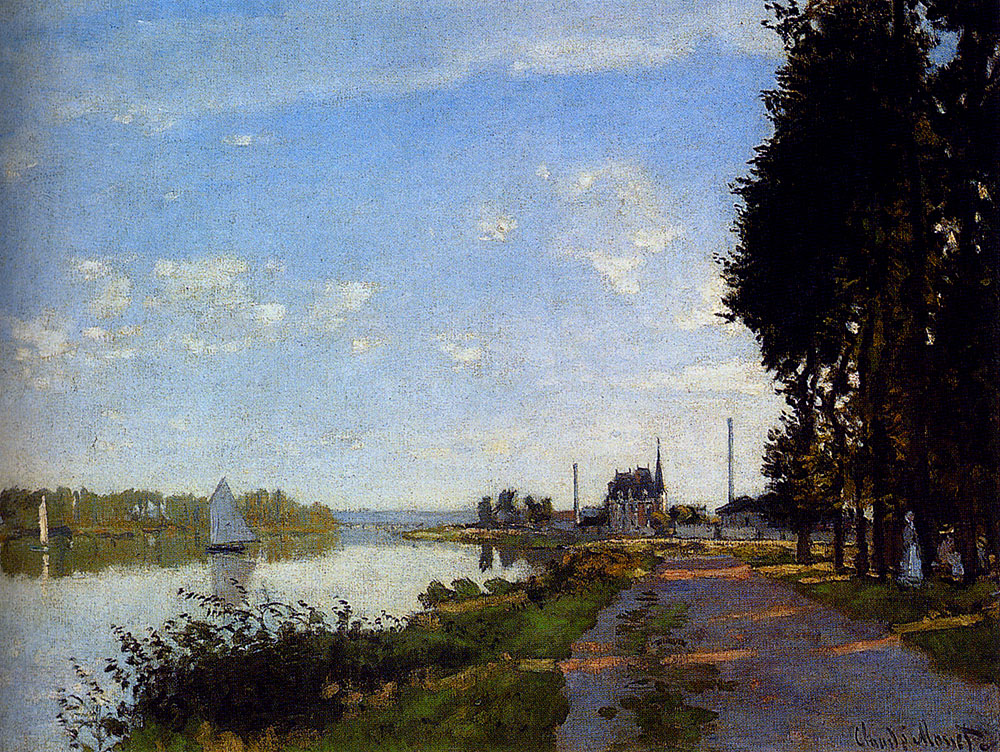
\includegraphics[height=5.5cm]{images/monet.jpg}}}
    \subfloat{{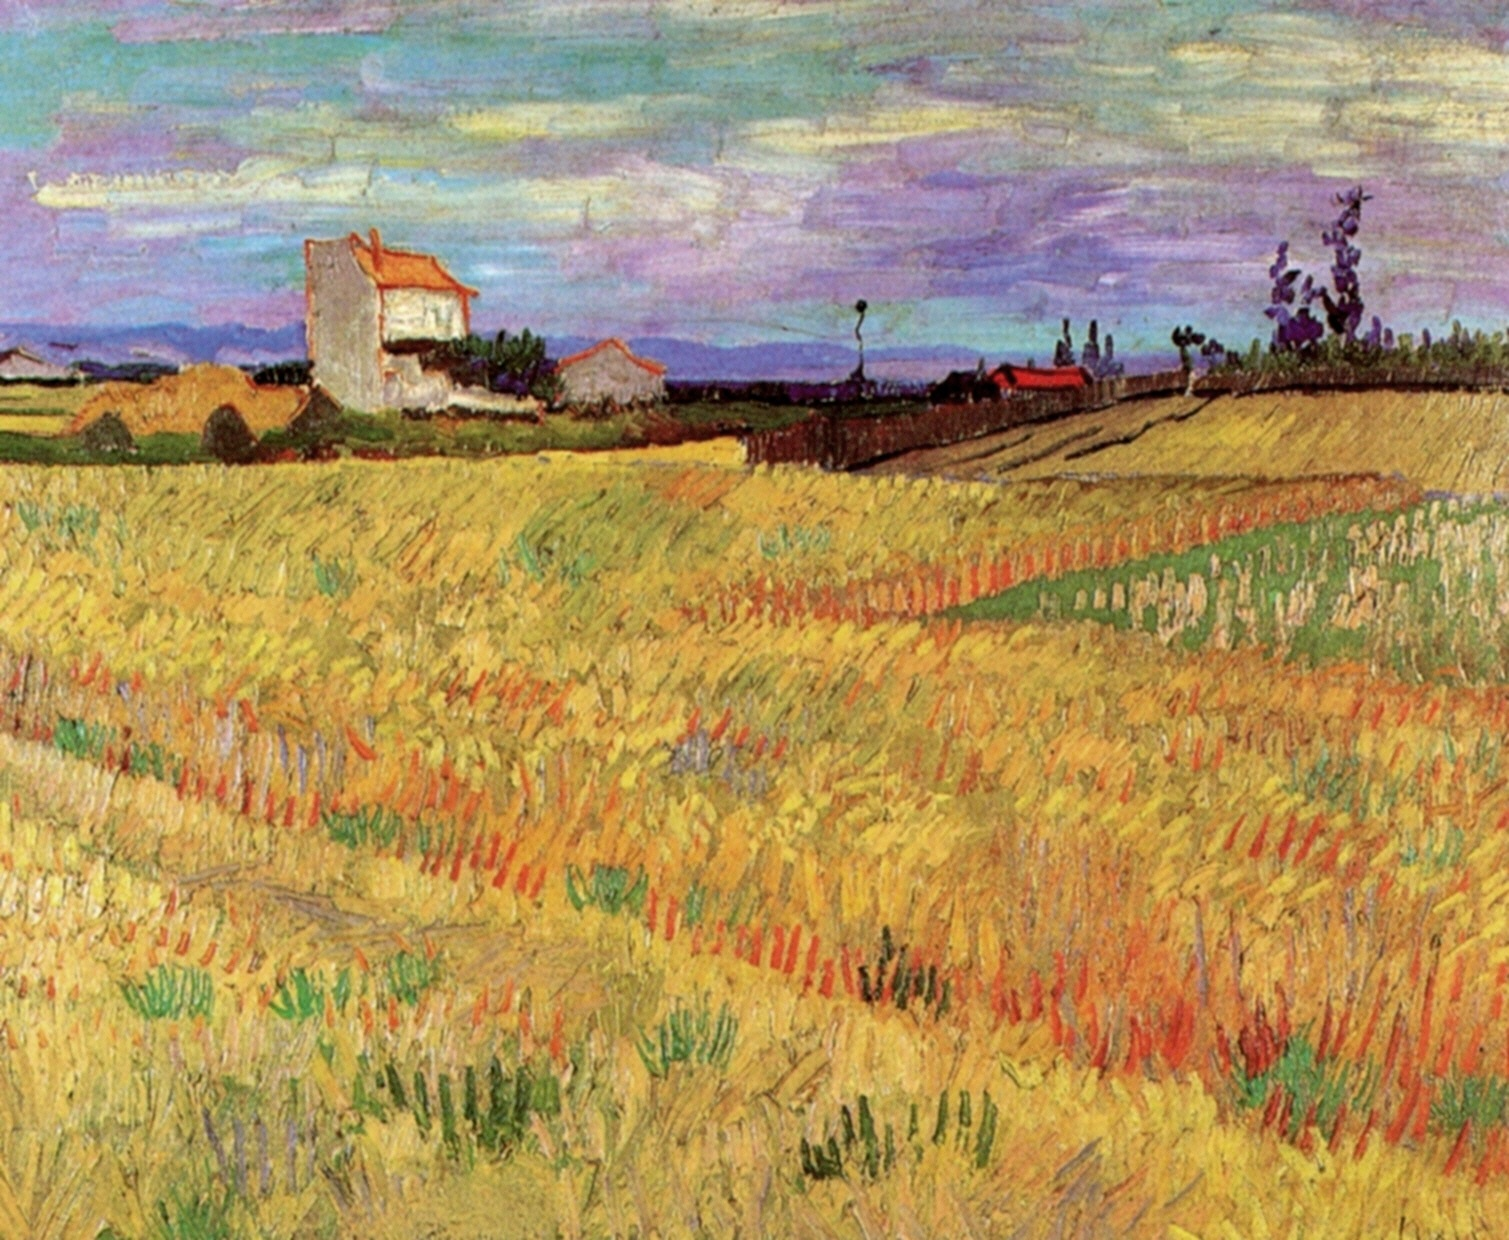
\includegraphics[height=5.5cm]{images/vangogh.jpg}}}
    \caption{Экземпляры картин из обучающей выборки (как вы уже поняли, слева - Клод Моне, справа - Ван Гог).}
    \label{fig:my_label}
\end{figure}{}

\section{Convolutional encoder}

Сложно поспорить с тем, что сверточные нейросети очень хороши в извлечении признаков из картинок. Для достижения лучшего качества мы обучили небольшую нейросеть, которую использовали как энкодер эмбеддингов для исходных картинок.

\subsection{Архитектура}

Мы использовали четыре сверточных слоя с возрастающим числом каналов (32, 64, 128, 256) и фильтрами 3х3 с последующими слоями субдискретизации (максимум, фильтр 2x2). Выход последнего сверточного слоя подвергается поканальному усреднению (global average pooling). Далее следуют 2 полносвязных слоя на 128 единиц, а всю конструкцию венчает полносвязный слой с Softmax на 10 классов. В качестве промежуточной активации использовалась LeakyRelu с параметром $\alpha = 0.1$. Подробно архитектуру можно увидеть на рис. 2.

\begin{figure}[H]
    \centering
    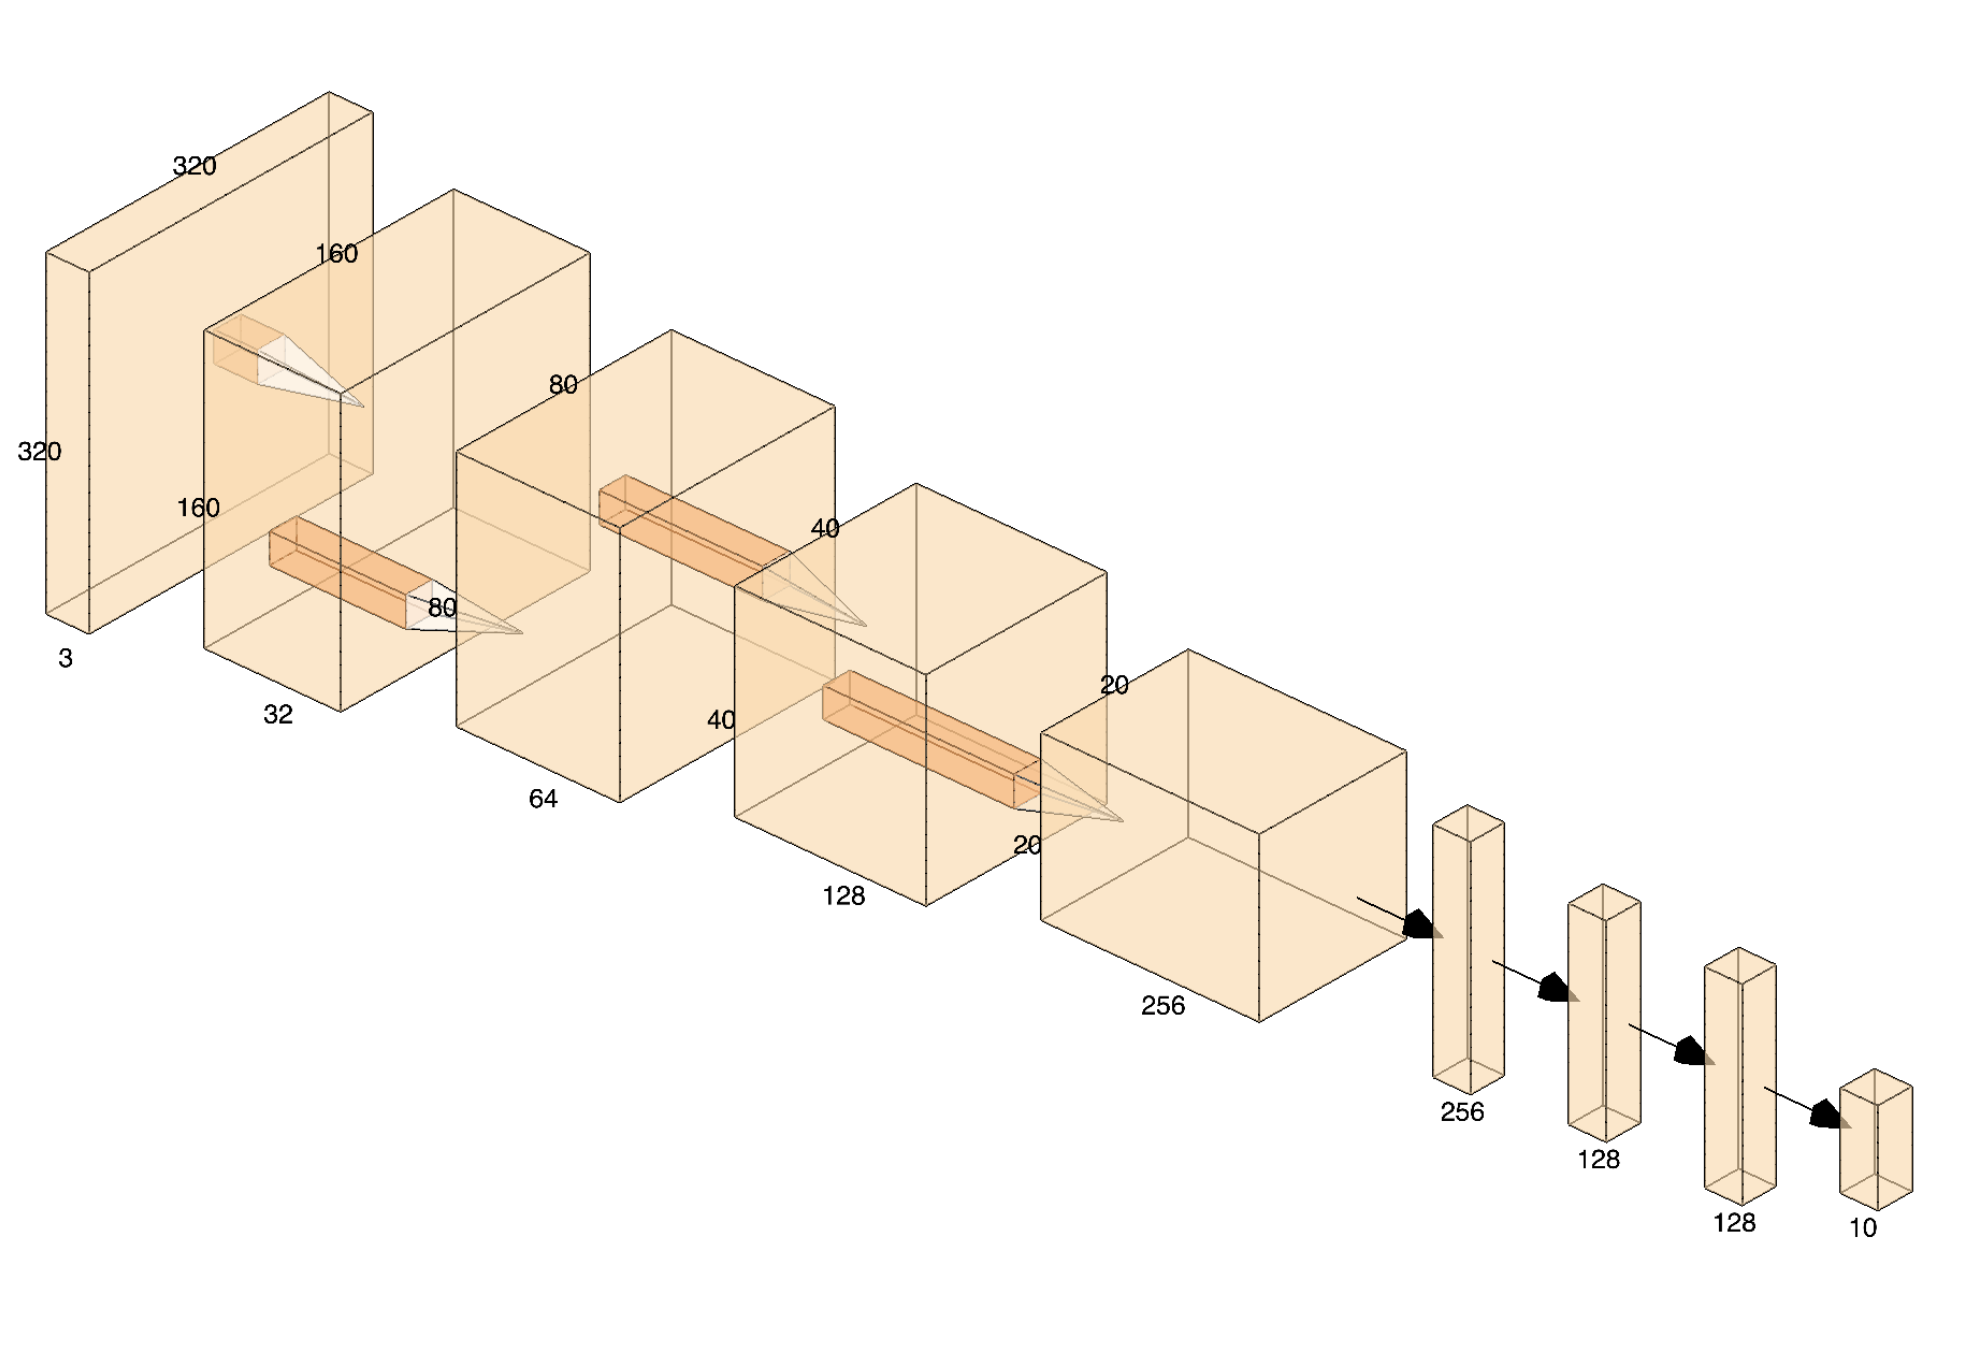
\includegraphics[width=14cm]{images/archirecture.png}
    \caption{Архитектура сверточного энкодера.}
    \label{fig:my_label}
\end{figure}{}

\subsection{Обучение}

Для подачи на вход сети картинки подгонялись под размер 320x320, в качестве функции потерь выступала категориальная кросс-энтропия. Для регуляризации сети использовался дропаут. Поскольку данных для задачи немного, аугментация хотя бы немного помогает от переобучения сети. Мы использовали нормальный шум, дисперсия которого увеличивалась на более поздних эпохах обучения. Еще один метод аугментации мы позаимствовали у \bibref{imclass}{}{Nitin Viswanathan}. Заключается он в том, что при обучении картинки случайно переворачиваются по горизонтали. В конце концов, сеть все равно получилась переобученной, но разрыв между качеством на обучающей и валидационной выборке оказался не столь разительным:

\begin{table}[H]
\centering

\begin{tabular}{M{2cm}|M{3cm}M{3cm}}
     & accuracy & top-3 accuracy \\
    \hline
    train & 0.644 & 0.891 \\
    test & 0.592 & 0.848 \\
\end{tabular}

\label{tab:my_label}
\end{table}

\subsection{Эмбеддинги}

В качестве эмбеддингов для картинок мы использовали выход последнего сверточного слоя (после поканального усреднения). Таким образом, получились вектора размерности 256. Их мы и использовали как основу для генерации случайных признаков.

\section{Эксперименты}

\subsection{Число признаков}

Мы провели серию экспериментов, в которой проверяли прирост качества от увеличения числа случайных признаков для разных ядер. Результаты убеждают в том, что модель имеет очень низкое смещение: она способна подгоняться под любые данные, что выражается в практически идеальном качестве на обучающей выборке.

Хуже всего себя показало ядро Лапласа (скорее всего это связано со свойствами распределения Коши, которое используется для аппроксимациии, в частности, у него отсутствует матожидание и дисперсия). Ядра Коши и Гаусса показали куда лучший результат с заметным превосходством последнего. В целом, качество ожидаемо растет с увеличением числа случайных признаков.

\begin{figure}[H]
    \centering
    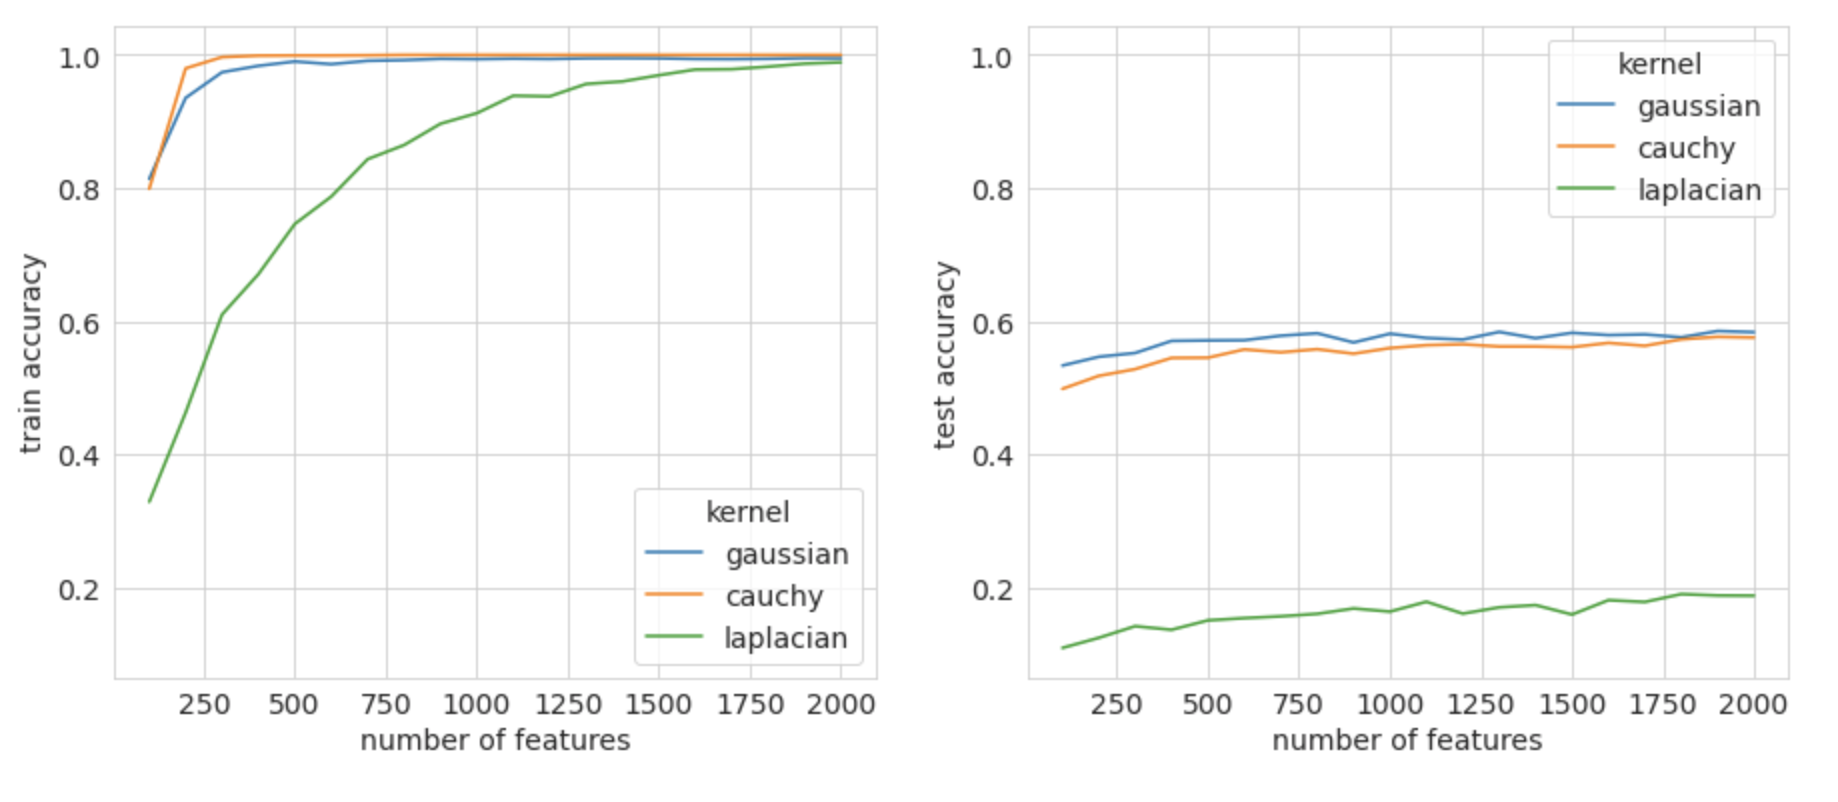
\includegraphics[width=14cm]{images/kernels_top1.png}
    \caption{Метрика accuracy для разных ядер при изменении числа признаков.}
    \label{fig:my_label}
\end{figure}{}

\begin{figure}[H]
    \centering
    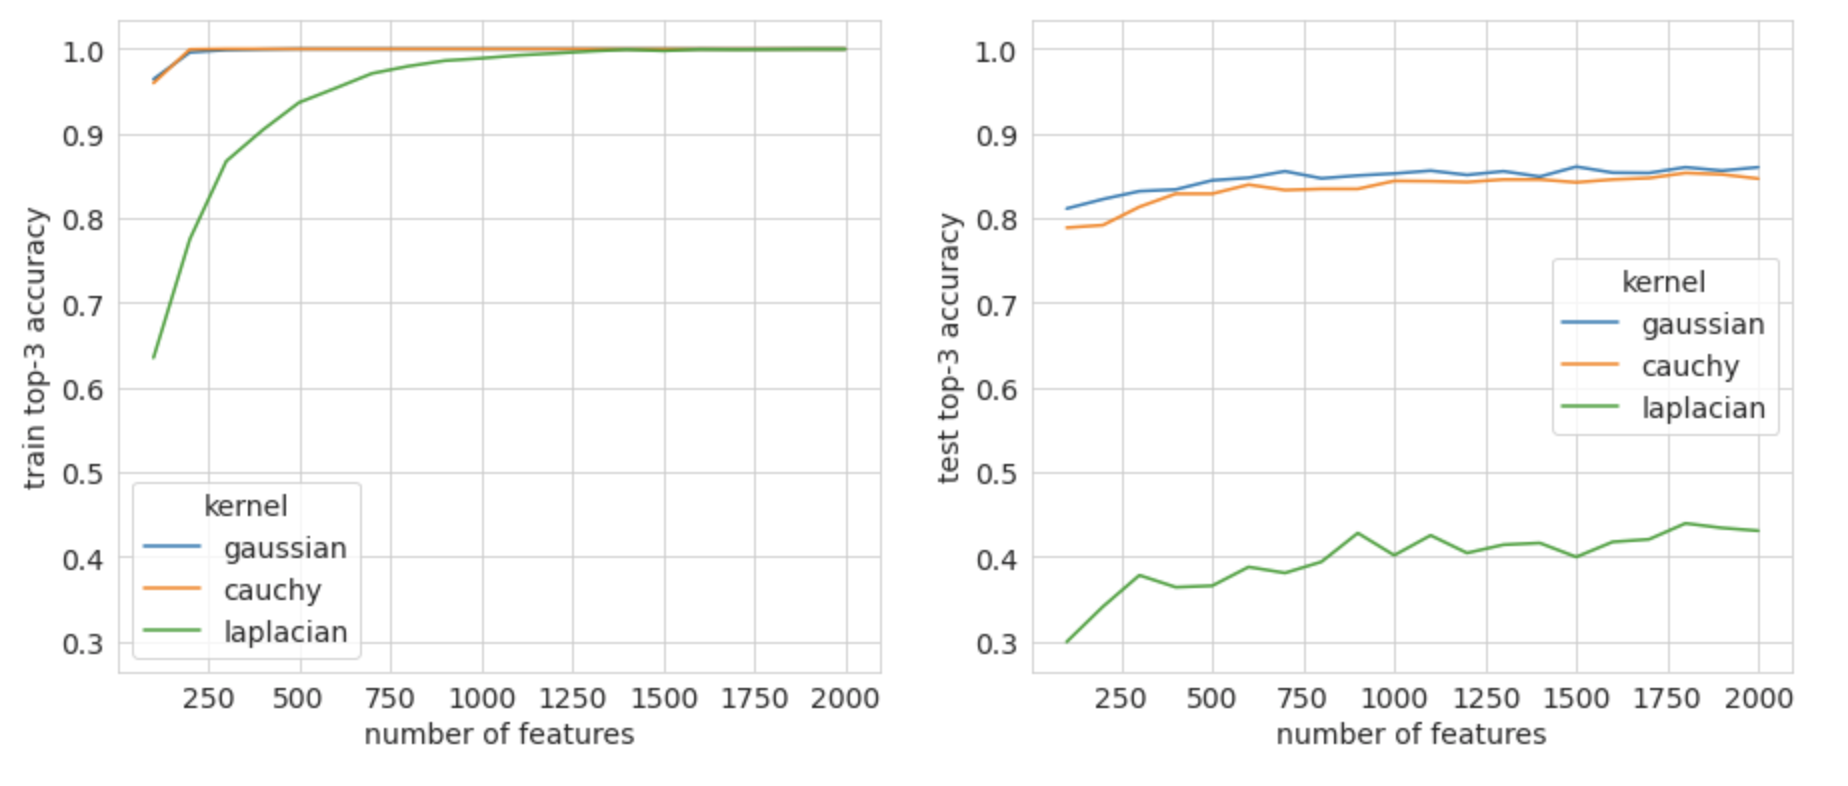
\includegraphics[width=14cm]{images/kernels_top3.png}
    \caption{Метрика top-3 accuracy для разных ядер при изменении числа признаков.}
    \label{fig:my_label}
\end{figure}{}

\begin{figure}[H]
    \centering
    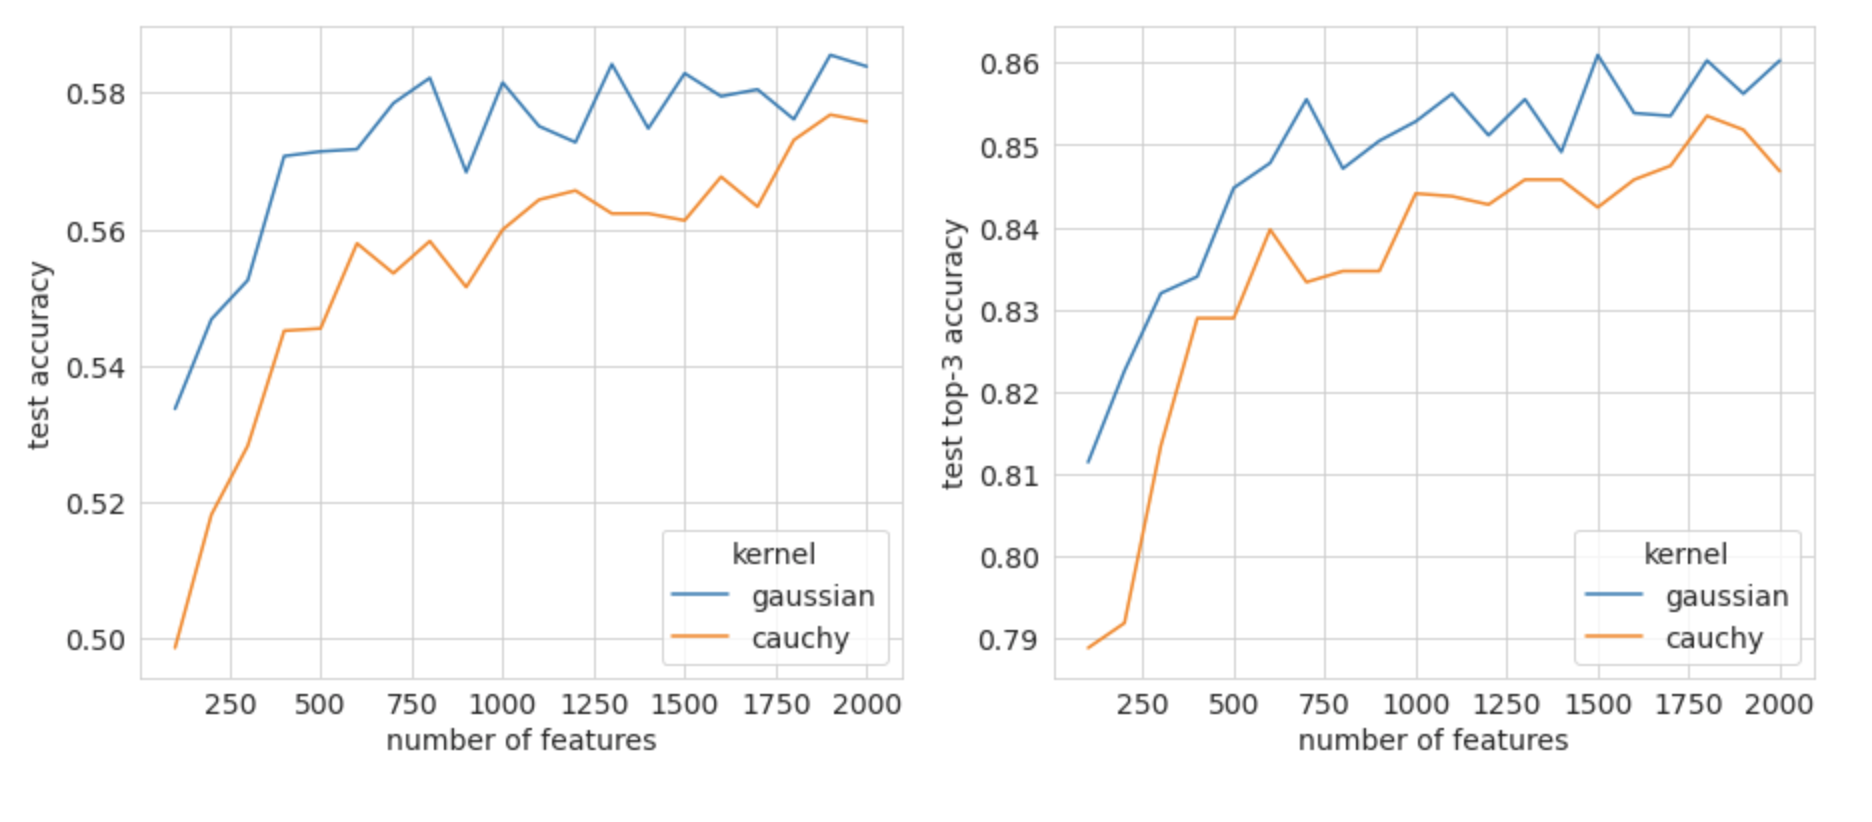
\includegraphics[width=14cm]{images/gauss_cauchy.png}
    \caption{Сравнение результатов для ядер Гаусса и Коши.}
    \label{fig:my_label}
\end{figure}{}

\subsection{Ортогональные признаки}

Мы провели эксперимент, который демонстрирует прирост качества при переходе от обычных случайных признаков к ортогональным. Сильнее всего этот эффект проявляется для небольшого числа признаков. Также любопытно, что при использовании ортогональных признаков понижается качество на обучающей выборки, так что ортогонализацию можно рассматривать как регуляризацию для случайных признаков.

\begin{figure}[H]
    \centering
    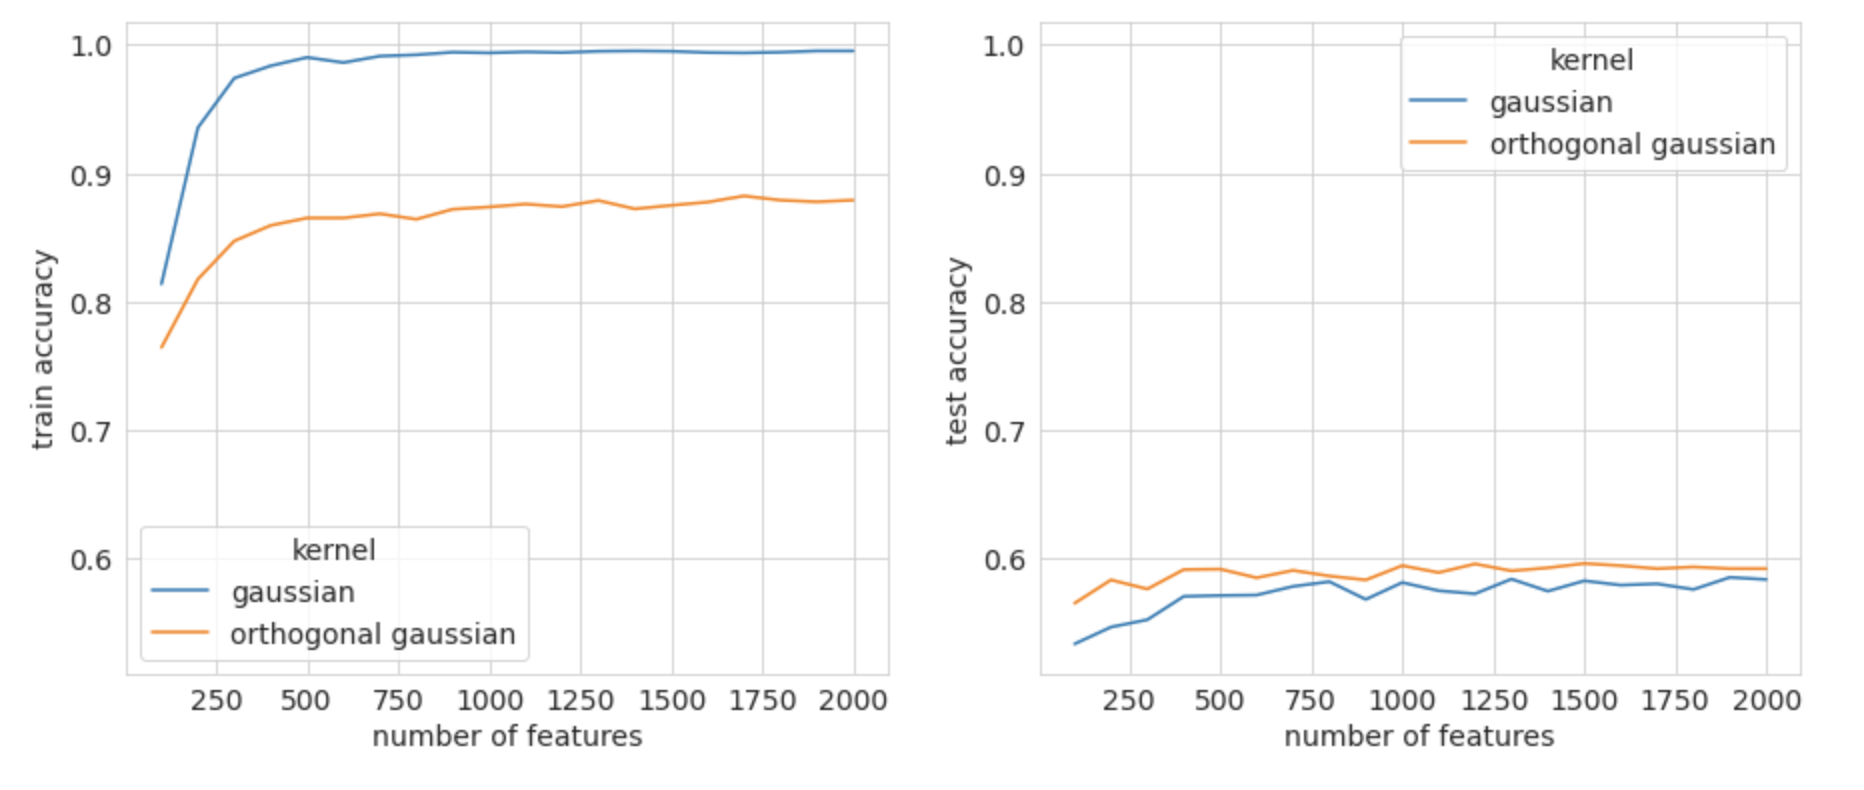
\includegraphics[width=14cm]{images/orthogonal_top1.png}
    \caption{Метрика accuracy для ядра Гаусса: обычные признаки против ортогональных}
    \label{fig:my_label}
\end{figure}{}

\begin{figure}[H]
    \centering
    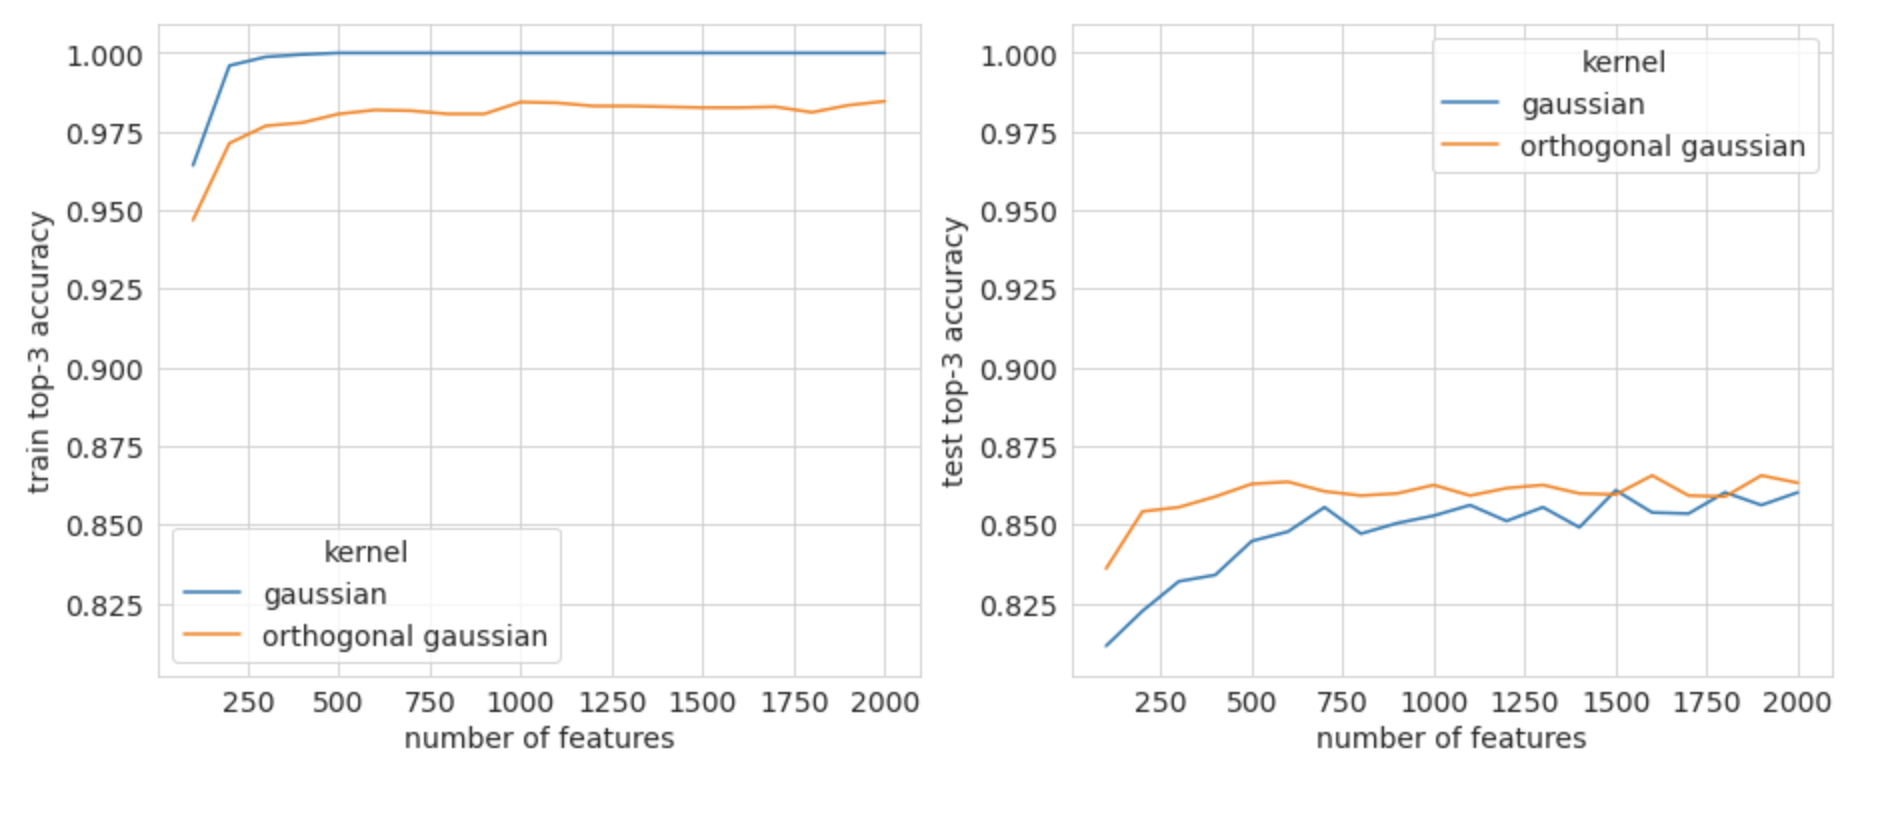
\includegraphics[width=14cm]{images/orthogonal_top3.png}
    \caption{Метрика top-3 accuracy для ядра Гаусса: обычные признаки против ортогональных.}
    \label{fig:my_label}
\end{figure}{}

\subsection{Регуляризация}

Еще один эксперимент показывает влияение коэффициента $\lambda$ на качество модели. На графиках видно, что качество модели на обучающей выборки растет при увеличении $\lambda$, при этом максимум качества на тестовой выборке приходится не на тривиальное значение $\lambda=1$, поэтому перебор $\lambda$ как гиперпараметра имеет смысл с точки зрения увеличения качества. Эксперимент подтверждает роль $\lambda$ как коэффициента регуляризации.

\begin{figure}[H]
    \centering
    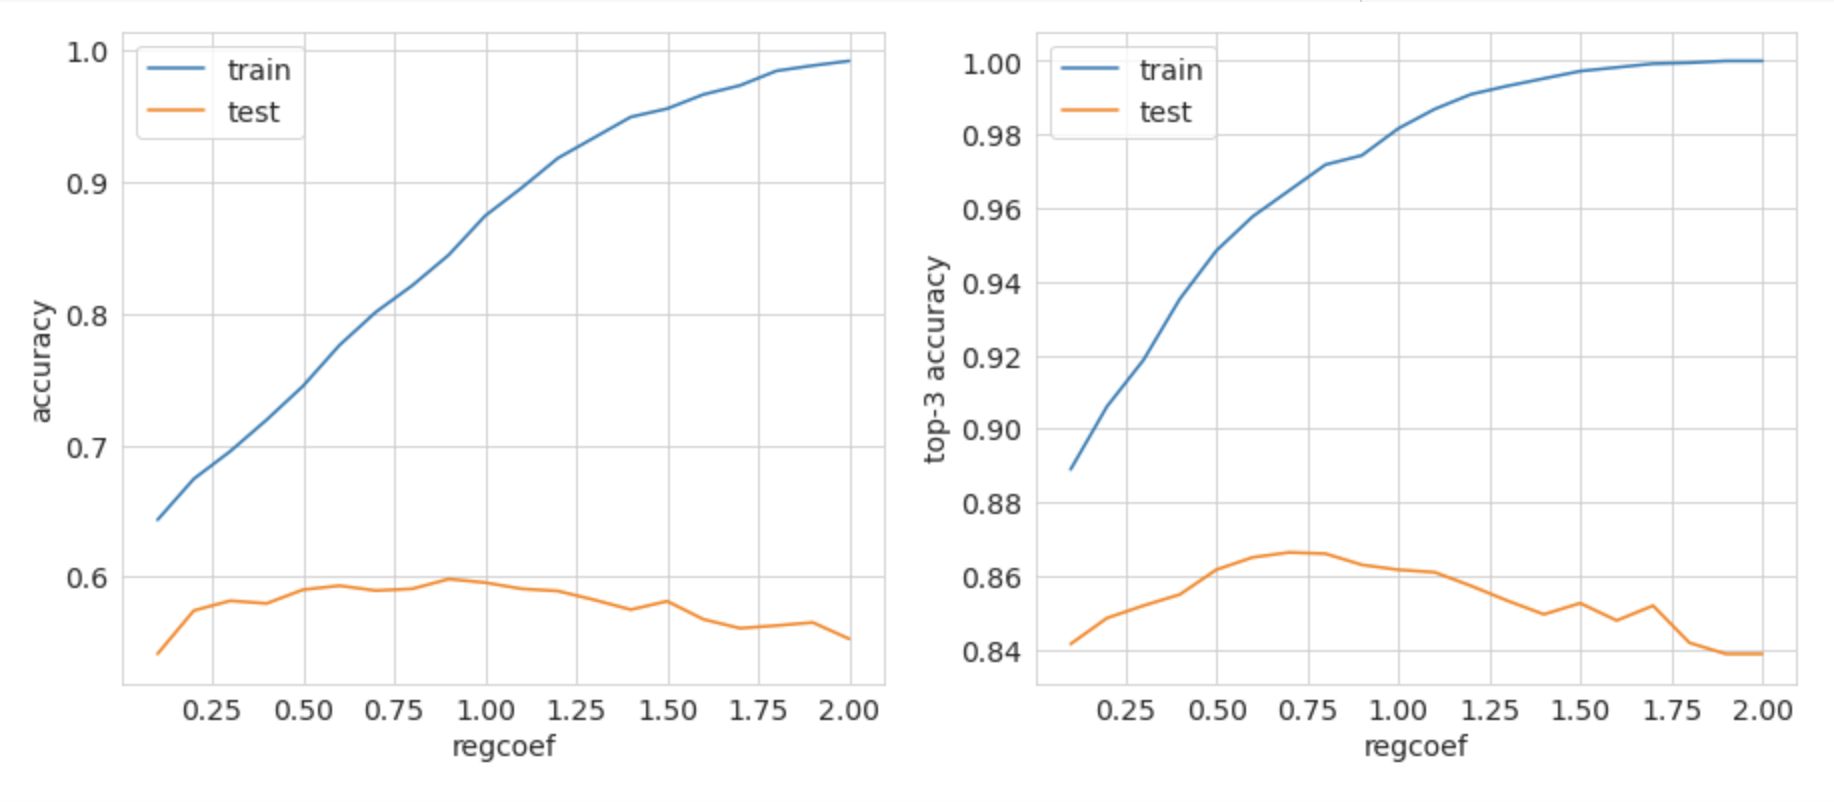
\includegraphics[width=14cm]{images/regcoef.png}
    \caption{Влияние коэффициента $\lambda$ на качество на обучающей и тестовой выборке.}
    \label{fig:my_label}
\end{figure}{}

\subsection{Результаты}

В качестве бейзлайна мы взяли логистическую регрессию и градиентный бустинг в реализации \bibref{lightgbm}{}{LightGBM}, которые применили к тем же самым эмбеддингам. Результаты на тестовой выборке представлены в таблице:

\begin{table}[H]
\centering

\begin{tabular}{M{2.5cm}|M{2.5cm}M{2.5cm}M{2.5cm}}
     & LogReg & LightGBM & ORF + LogReg \\
    \hline
    accuracy & 0.649 & 0.633 & \textbf{0.674} \\
    top-3 accuracy & 0.892 & 0.864 & \textbf{0.900} \\
\end{tabular}

\label{tab:my_label}
\end{table}

\noindent
Такого результата удалось добиться при использовании ортогональных гауссовских признаков при значениях параметров $D=4000, \lambda=0.85$. Стоит заметить, что результат сильно варьировался от запуска к запуску, но всегда был выше, чем у логистической регрессии. Таким образом, использование случайных признаков привело к приросту качества на 2\%.

\bigskip

\noindent
\textsc{А теперь посмотрим, как не стоит использовать Random Fourier Features}

\section{Какие еще эмбеддинги}

Зачем нам эти сложности с обучением каких-то нейронных сетей? Просто возьмем картинки и представим их в виде вектора размерности $224 \times 224$. (Обратим внимание, что канал использовался только один, 3 канала уменьшали качество и требовали больше времени и памяти). После применения к ним PCA разложения в теории должны остаться только самые важные пиксели, так что такого размера не стоит пугаться.

\subsection{Опять эксперименты}

Обычная логистическая регрессия к таким данным смогла добиться результата в 24\%, что значительно уступает обучению на эмбеддингах. 

\begin{figure}[H]
    \centering
    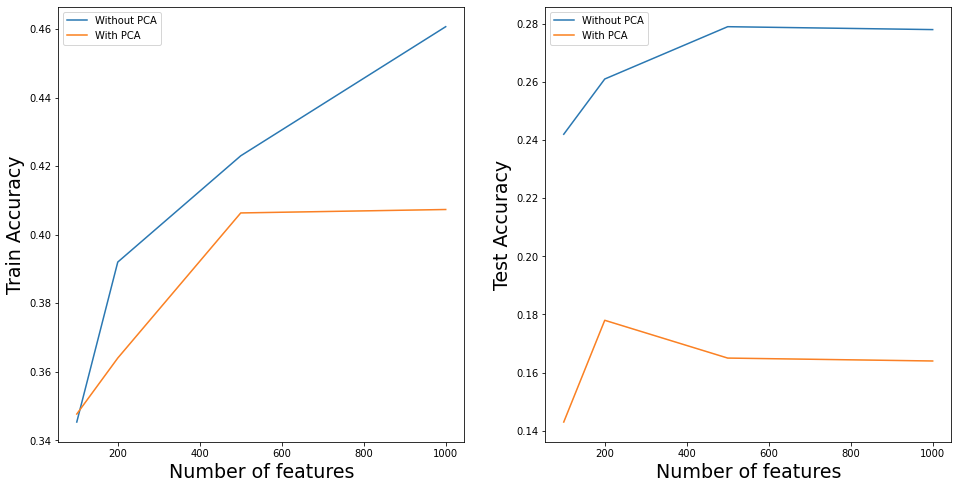
\includegraphics[width=12cm]{images/cauchy_pca_diff.png}
    \caption{Влияние числа признаков на качество на обучающей и тестовой выборке при использовании PCA с размерностью 100.}
    \label{fig:my_label}
\end{figure}{}


\begin{figure}[H]
    \centering
    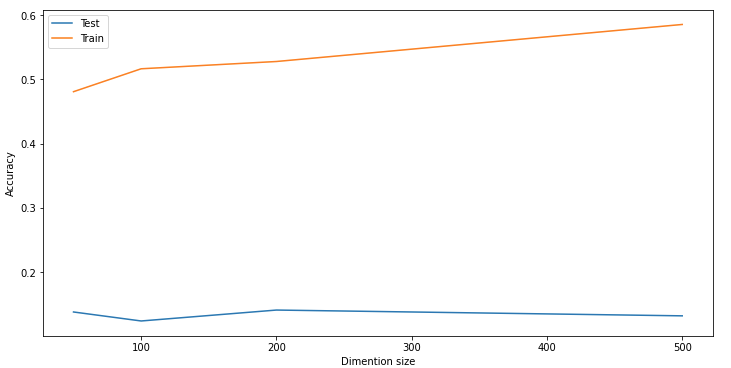
\includegraphics[width=12cm]{images/n_dim_simple.png}
    \caption{Влияние размерности PCA на качество на обучающей и тестовой выборке.}
    \label{fig:my_label}
\end{figure}{}

Как мы видим, PCA не может дать хорошую базу признаков для RFF, поэтому качество получается посредственное даже для тренировочной выборке. На наш взгляд, дело в специфике задачи. Стиль художника практически невозможно выразить небольшим количеством пикселей, как это можно сделать в задачах классификации объектов на картинке. Для него необходимо смотреть на всю картину, а также извлекать более сложные признаки. В качества плюса можно отметить только ускорение обучения, ведь признаков стало не 50 тысяч, а примерно 1000, но при качестве, близком к качеству случайных предсказаний, это сомнительный плюс.

\bigskip

Возможно, ортогональные признаки как-то смогут исправить ситуацию?

\begin{figure}[H]
    \centering
    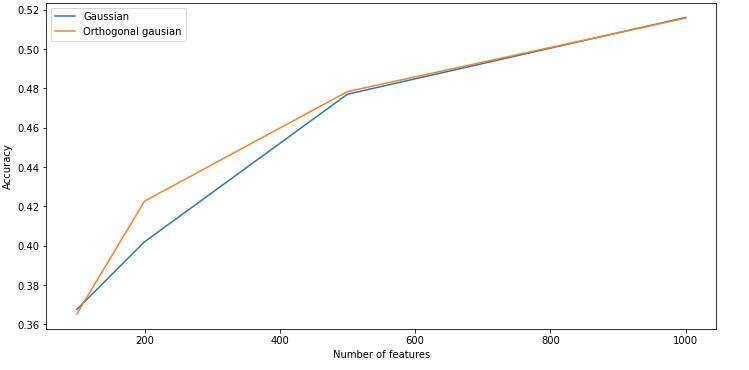
\includegraphics[width=7cm]{images/orthogonal_train.jpg}
    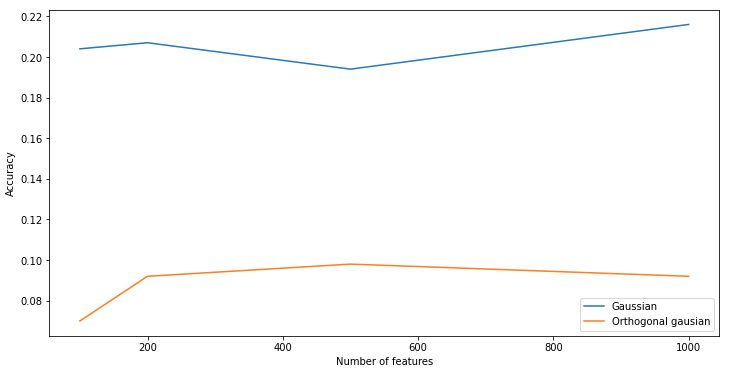
\includegraphics[width=7cm]{images/orthogonal_test.png}
    
    \caption{Качество при использовании ортогональных признаков на тренировочной и тестовой выборках}
    \label{fig:my_label}
\end{figure}{}

Нескореллированные признаки это, конечно, хорошо, но когда они не очень хорошие, это не может помочь. Из забавного: ортогонализация действительно работает как регуляризация и замедляет обучение. Увы, признаки настолько плохие, что ничего не выучилось.

\section{Классификация текстов}

А что же у нас с классификацией текстов? Для анализа был взят датасет с заголовками статей с \bibref{medium}{}{Medium.}

\subsection{Данные}
Данные состояли из заголовков и подзаголовков постов, по которым необходимо было определить тематику статьи: одну из 92. Текст преобразовался с помощью tf-idf.

\subsection{Эксперименты}

Простой логрег выбивает на таком 43\% точности. Попробуем улучшить это с помощью силы рандома.

\begin{table}[H]
\centering

\begin{tabular}{M{2.5cm}|M{2.5cm}M{2.5cm}M{2.5cm}}
     & Gaussian & Laplacian & Cauchy \\
    \hline
    train & 0.67 & 0.94 & 0.85 \\
    test & 0.28 & 0.17 & 0.29 \\
\end{tabular}

\label{tab:my_label}
\end{table}

Давайте, пожалуйста, забудем про эти попытки применить RFF к текстам в таком виде. Казалось, что tf-idf может дать нормальную базу и мы получим какие-то ключевые слова с помощью PCA. Но нет, не получим, так как судя по всему у нас будет просто много слов общего смысла, которые часто употребляются. Из-за этого в большинстве случаев логрег не может сойтись, но что-то да выучивает (подозреваю, что 1-2 самых популярных класса).

Также была попытка накинуть на все это 1d свертки перед логрегом, но они все же предназначены для последовательностей, поэтому вышло еще хуже.

\section{Вывод}

Что можно сказать в конце. RFF --- это неплохой способом добыть признаки, если есть хорошая база, а также может являться одним из видов регуляризации. Невероятных высот с помощью такого применения рандома добиться вряд ли получится, но добить последние несколько процентов точности вполне можно, если использовать этот алгоритм с умом.

\begin{figure}[H]
    \centering
    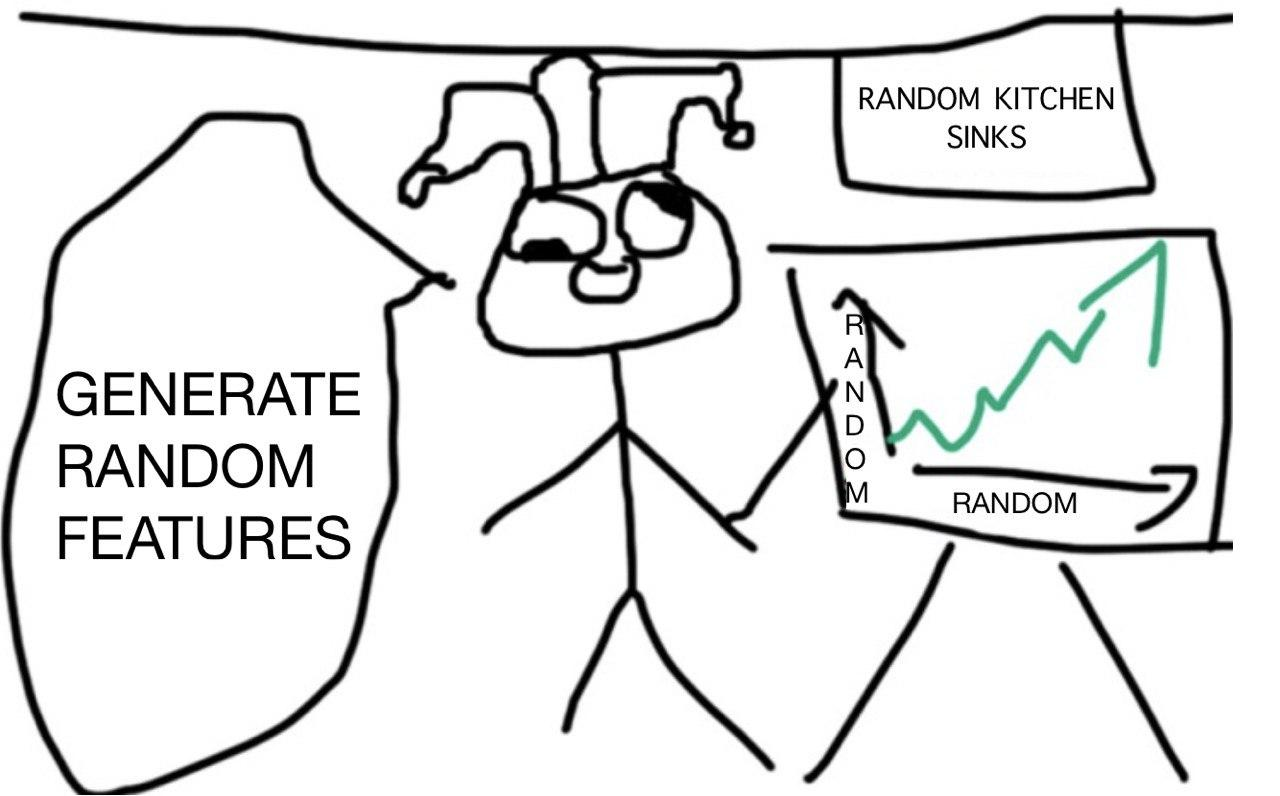
\includegraphics[width=14cm]{images/meme.jpg}
    
    \caption{Спойлер: так ничего не заработает}
    \label{fig:my_label}
\end{figure}{}

\newpage
\section{Список источников} 
\begingroup
\renewcommand{\section}[2]{}
\begin{thebibliography}{}

\bibitem{kaggle}\hypertarget{kaggle}{}
\textit{Panchajanya Banerjee (Pancham)}. Impressionist classifier data. URL: 
\url{https://www.kaggle.com/delayedkarma/impressionist-classifier-data}, свободный (дата обращения: 03.06.2020).

\bibitem{imclass}\hypertarget{imclass}{}
\textit{Nitin Viswanathan}. Artist Identification with Convolutional Neural Networks

\bibitem{kernels}\hypertarget{kernels}{}
\textit{Ali Rahimi, Benjamin Recht}. Random Features for Large-Scale Kernel Machines.

\bibitem{orf}\hypertarget{orf}{}
\textit{Felix Xinnan Yu et al}. Orthogonal Random Features.

\bibitem{lightgbm}\hypertarget{lightgbm}{}
\textit{Microsoft Corporation}. LightGBM documentation. URL: \url{https://lightgbm.readthedocs.io/en/latest}, свободный (дата обращения: 04.06.2020).

\bibitem{medium}\hypertarget{medium}{}
\textit{amrrs}. Medium post titles. URL: 
\url{https://www.kaggle.com/nulldata/medium-post-titles}, свободный (дата обращения: 31.05.2020).


\end{thebibliography}{}
\endgroup

\end{document}
